\section{Versuchsaufbau}
%skizze zum versuchsaufbau (oder foto) einf�gen,   es muss erkl�rt werden wie das ganze funktioniert und welche speziellen einstellungen verwendet wurden (z.b. welche kn�pfe an den ger�ten f�r die messung verdreht wurden)
Der Versuchsaufbau befindet sich ein einem Kasten aus Bleibl�cken. Als Quelle f�r die $\gamma$-Strahlung wird eine Caesium verwendet. Der Detektor und die Probe sind auf einer drehbaren Halterung montiert. Bei dem Detektor handelt es sich um ein NaI-Szintillator, das Signal wird mit Photomuliplier verst�rkt und �ber die Ausleseelektronik an die Computer weitergeleitet. Die Effizienz des Detektors in Abh�ngigkeit der Photonenenergie ist in Abb. \ref{fig:effizienz} zu sehen. 

\begin{figure}[H]
\centering
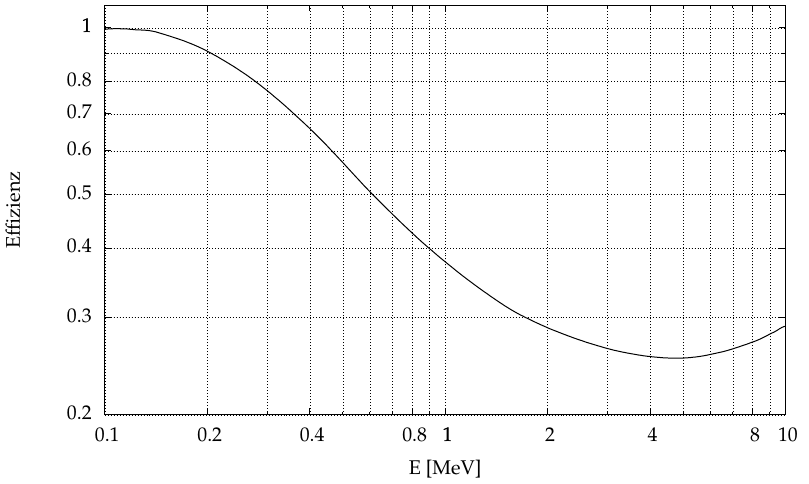
\includegraphics[scale = 0.39]{effizienz.png}
\caption{Effizienz des Detektors in Abh�ngigkeit der Energie des eintreffenden Photons, entnommen von \cite{Versuchsanleitung}}
\label{fig:effizienz}
\end{figure}

Hinter der Probe befindet sich die Quelle. Eine Skizze des Versuchsaufbaus ist in Abb. \ref{fig:aufbau} zu sehen . 

\begin{figure}[H]
\centering
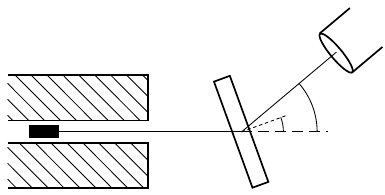
\includegraphics[scale = 0.7]{aufbau.png}
\caption{Schematischer Aufbau des Versuchs, entnommen von \cite{Versuchsanleitung}}
\label{fig:aufbau}
\end{figure}

F�r die Verst�rkung des Signals wurde eine coarse-gain von 50 eingestellt, die fine-gain wurde mit 7,3 eingestellt und der conv-gain wurde auf ein 0.5 eingestellt. Der Photomuliplier wurde mit einer Spannung von 650V betrieben.

